\documentclass[12pt]{article}

\usepackage[UTF8]{ctex}
\usepackage[margin=1in]{geometry}
\usepackage{amsmath,amssymb,amsthm}
\usepackage{array,booktabs,longtable,tabularx}
\usepackage{graphicx}
\graphicspath{{}{mcm2027-b-phoenix-cooling/}}
\usepackage{float}
\usepackage{setspace}
\usepackage{indentfirst}
\usepackage{needspace}
\usepackage{fancyhdr}
\usepackage{lastpage}
\usepackage{enumitem}
\usepackage[table]{xcolor}
\usepackage{titlesec}
\usepackage[font=normalsize,labelfont=bf]{caption}
\usepackage[numbers,sort&compress]{natbib}
\usepackage{xurl}
\usepackage{hyperref}

\hypersetup{colorlinks=true,linkcolor=black,citecolor=black,urlcolor=black}
\setstretch{1.0}
\setlength{\parindent}{1.5em}
\setlength{\parskip}{0pt}
\setlength{\emergencystretch}{3em}
\setlist{nosep,leftmargin=1.6em}
\renewcommand{\arraystretch}{1.15}
\newcommand{\teamcontrol}{队伍控制号待填}
\newcommand{\solutionpages}{\pageref{solutionlastpage}}
\newcommand{\OBS}{\textnormal{[观测]}}
\newcommand{\MODEL}{\textnormal{[模型]}}
\newcommand{\ASSUME}{\textnormal{[假设]}}
\newenvironment{summary}{}{\clearpage}

\pagestyle{fancy}
\fancyhf{}
\fancyhead[L]{\fontsize{12}{14}\selectfont\teamcontrol}
\fancyhead[R]{\fontsize{12}{14}\selectfont 第\thepage\ 页 / 共 \solutionpages\ 页}
\renewcommand{\headrulewidth}{0.4pt}
\setlength{\headheight}{15pt}
\raggedbottom
\titleformat{\section}{\Large\bfseries\color{black}}{\thesection}{0.6em}{}
\titleformat{\subsection}{\large\bfseries\color{black}}{\thesubsection}{0.55em}{}
\titleformat{\subsubsection}{\normalsize\bfseries\color{black}}{\thesubsubsection}{0.5em}{}
\titlespacing*{\section}{0pt}{1.15em}{0.45em}
\titlespacing*{\subsection}{0pt}{0.75em}{0.25em}
\titlespacing*{\subsubsection}{0pt}{0.5em}{0.15em}

\begin{document}

\begin{summary}
\begin{center}
    {\fontsize{24}{28}\selectfont\bfseries 从可达缺口到韧性部署\par}
    \vspace{0.25em}
    {\Large\bfseries 凤凰城移动降温枢纽的公平规划与运营策略\par}
    \vspace{0.8em}
    {\normalsize\bfseries 摘要\par}
\end{center}
\vspace{0.35em}

2025 年 Phoenix 的一周降温服务记录了 3,929 次访问，但已实现访问量会被营业时间、容量与出行选择共同截断，不能直接代表所有潜在需求。本文因此把问题改写为：在这些不确定因素下，空间布局、服务时段与移动资源分别会怎样改变可服务的人次？我们先用人口、热暴露和脆弱性构造区间相对需求，再以该观测周总量校准情景规模；随后将营业窗口、可达性和容量接入同一分配模型，并延伸到选址、七日调度、故障响应与五年预算规划。所有结果均为条件情景，不是 Phoenix 居民的实测覆盖率。

校准后的七日基准总需求约为 3,929 人次；首日为 505.0 人次，其余日期按预设热浪因子变化。合成网络中增加 3 台 MCH 后，模型缺口由 305.511 降至 227.295 人次/日，但需求放大或分群比例变化会改变选址。加入 MAG 站点与日期化来源日历后，另一个交通代理情景的缺口为 212.768 人次/日。两项都是同一需求量级下的模型比较，并非现场服务验证。

七日比较给出一个反直觉结果：若需求只按全区共同因子变化，搬迁没有收益；只有局部需求冲击改变空间排序时，模拟搬迁才减少缺口。这个发现把建议从“多买车”转向先核实夜间服务、真实出行和人员条件。应急压力测试与五年预算结果同样依赖明示的离散假设和情景成本，因此仅用于设计试点和后续测量。

结果支持把固定中心延时和真实服务数据采集列为优先评估事项，再决定移动试点规模。输入来源与代码测试已有核验，但独立的区日潜在需求、逐站真实容量、现场 OD、人员成本和留出服务结果仍缺，因此本文提供的是可复算条件情景与采样方案，不是实际覆盖率预测、健康因果结论或采购承诺。

\vspace{\baselineskip}
\noindent\textbf{关键词：} 移动降温枢纽；选址—分配；服务可达性；公平性；动态调度；中断响应
\end{summary}

\clearpage
\renewcommand{\contentsname}{目录}
\setcounter{tocdepth}{2}
\begingroup
\titleformat{\section}{\centering\Large\bfseries\color{black}}{}{0pt}{}
\tableofcontents
\endgroup

\clearpage
\section{引言}

\subsection{研究背景}
持续高温下，安全的室内降温空间是公共服务网络的一部分。Phoenix 2025 热季至少有 37 天最高温度达到 110$^\circ$F，23 个夜晚最低温度不低于 90$^\circ$F [F07,F10]\citep{phoenixplan}。同季市级报告累计记录 44,508 次服务访问 [F11]\citep{weeklyreport}。这些访问是重复计数的人次，并不等于独立受益人数。Maricopa County 的访客调查显示，交通和开放时间都是已到访者报告的障碍；但该样本存在选择效应，不能直接代表所有居民\citep{maricopasurvey}。

Phoenix 的 Heat Relief Network 包含休息中心、降温中心、饮水站和其他合作点。设施类型决定其能否提供空调室内空间，因此不能把饮水站的数量当作降温容量\citep{phoenixplan}。固定设施也可能无法覆盖所有地区或晚间时段。移动降温枢纽可以补充固定网络，但车辆的旅行、搭建、人员和停服会减少当日有效服务。

\subsection{研究问题与贡献}
本文按赛题五问建立一致的需求—供给—分配链。Q1 描述固定网络缺口；Q2 评估移动枢纽数量、选址和公平；Q3 比较七日固定与动态调度；Q4 在同一事故输入下比较不搬与重新部署；Q5 在年度预算和资产约束下比较五年路径。本文的贡献是把设施类型、营业日历、到达时间和服务人次放入同一口径，并明确区分数值算法验证与现实服务验证。

\section{问题重述与建模路径}
题目允许使用公开数据，也允许在无法匹配观测数据时构造明确记录的模拟区—站网络。我们把 12 区、8 个移动候选点和每台每日最多 250 visitor-visits 作为测试规模；它们均为竞赛假设，不是官方凤凰城边界、批准站址或实测容量\citep{mcm2027b}。移动枢纽被视为对既有网络的补充，而非替代。

本文严格区分四类量：饮水服务与室内降温服务；每日访问人次、独立人数与同时在场人数；热相关死亡统计与设施因果效应；模拟规划区与官方行政边界。我们的优化输出是条件服务量与未满足需求，不推断减少了多少急诊、住院或死亡。

\section{数据与证据口径}

\subsection{观测资料与模型输入}
Phoenix 2026 Heat Response Plan 提供设施类别、政策行动和季节背景；2025 周报提供已实现访问量；访客调查用于说明到访者报告的交通和营业时段障碍；MAG 2026 公共视图提供站点位置、类别及来源登记营业字段\citep{mag}；Valley Metro 两版 GTFS 快照的有效期分别为 2026-04-27--07-26 和 2026-07-27--10-25\citep{gtfs}。本文没有使用排班 GTFS 计算门到门 OD，而使用有明确标签的距离/速度代理。官方人口计数来自 Phoenix HSD 对 ACS 2018--2022 的报告汇总\citep{acs}。原件、获取日期、哈希和转换记录见仓库数据说明\citep{modelrepo}。

\begin{table}[H]
\centering
\caption{主要数据与用途}
\begin{tabularx}{\textwidth}{p{0.23\textwidth}p{0.34\textwidth}X}
\toprule
资料 & 可核验内容 & 本文用途及边界 \\
\midrule
Phoenix 2025 周报 & 热季 44,508 次访问；9 月 4--10 日周合计 3,929 次 & 校准模拟七日总量；不等于潜在需求或未满足需求 \\
Maricopa 访客调查 & 15 个中心的访客交通和服务障碍 & 选择出行/时段情景；不能代表全市居民比例 \\
MAG 2026 公开视图 & 50 个登记点：24 个降温点、26 个饮水点 & 现有设施位置与逐日营业字段；不含逐站真实容量 \\
GTFS 快照 & Valley Metro 两版静态时刻表，有效期 2026-04-27--10-25 & 做源数据核验；本文不称其为排班 OD \\
官方 15 村人口资料 & 人口、户数和年龄计数，可按映射聚合 & 检查聚合输入；12 个规划区仍为竞赛模拟区 \\
\bottomrule
\end{tabularx}
\end{table}

\subsection{资料状态与验证范围}
MAG 原始字段、站点 ID 与逐星期日历规则已完成来源重构核验；350 个站点—日期格中，267 格有明确钟点、76 格未知、7 格处于来源季节范围外。旧 weekday 包络对明确钟点的端点平均绝对误差为 0.279 小时，逐日来源重构误差为 0。该零误差是同一来源字段的程序重构结果，不是独立观测，也不证明设施实际开门。当前没有含被拒绝需求的区—日请求、逐站实测容量/营业和匹配出行路线，故以下结果只作条件情景比较。

\section{假设与符号}

\subsection{主要假设}
\begin{enumerate}[label=\textbf{A\arabic*.}]
    \item \textbf{12 区映射。}题目需要有限规划区；将 15 个官方 urban villages 聚合到 12 个模拟区以满足该结构，但映射并非官方行政边界。该映射进入需求权重与区—站链接 $a_{ij}$；边界改变会改变空间需求和选址，须用替代映射重算。
    \item \textbf{潜在需求与总量。}逐区相对权重由人口、热暴露和脆弱性构造，再以 2025-09-04 至 09-10 已实现访问总量校准一周总量；这样可给无完整需求调查的模型一个可追溯量级。访问量受容量和选择影响，校准不等于识别潜在需求，故需求率与地区比例须作情景参数，并以留出热浪验证。
    \item \textbf{分群及时间份额。}housed/unsheltered 基础需求比例取 50/50，分时份额分别为日/晚/夜 0.55/0.38/0.07 与 0.30/0.45/0.25；这是把开放时间与需求放入同一约束的必要输入，不是从访客样本外推的人口比例。它进入 $D_{ith}$；份额变化会改变时段供需匹配，故报告 0.5--0.7 等份额敏感性。
    \item \textbf{站点容量与吞吐。}MAG 未发布逐站日接待量，固定站的 50 人次/日和窗口内均匀吞吐率是可计算的工作假设；MCH 的 250 人次/日来自题设。它们进入式\,(\ref{eq:capacity})及容量约束。容量从 20 到 50 人次/日已导致点集改变；应以席位、停留时长、工作人员和实际计数替换。
    \item \textbf{可达时间。}没有已匹配的门到门出行记录，故以区代表点、坐标距离、绕行系数 1.35、步行速度 4.8 km/h、公交代理速度 15 km/h 加 10 分钟等待构造链接；这是形成可行边 $A_{ij}$ 的必要近似，不是 GTFS 路由。距离/速度偏差可能双向改变可达集合，应以同日 GTFS OD 与现场路线校验。
    \item \textbf{未知营业时段。}76 个空白站点—日期格按零供给保守处理，避免把未知误算为开放；该政策进入式\,(\ref{eq:capacity})，也可能低估服务。补采机构逐日营业表后应与“未知按开”上界配对，而不得把空白当作已证实关闭。
    \item \textbf{故障与投资。}Q4 抽样故障、需求/出行/搬迁倍率和 Q5 车辆、运营、延时、预算均为明示情景，因为缺乏本地连续故障与报价数据；它们分别进入 $G$ 和年度成本约束。若真实报价、道路或配员超出扫描范围，当前排序失效，须先收集本地报价、交期、合同、人员和许可，再重算。
\end{enumerate}

\subsection{符号说明}
\begin{longtable}{>{\centering\arraybackslash}p{0.20\textwidth}p{0.58\textwidth}p{0.12\textwidth}}
\caption{主要符号}\label{tab:notation}\\
\toprule 符号 & 定义 & 单位 \\
\midrule
\endfirsthead
\toprule 符号 & 定义 & 单位 \\
\midrule
\endhead
$i\in I$ & 12 个模拟规划区索引 & -- \\
$j\in J$ & 固定服务点或 MCH 候选点 & -- \\
$t\in\{1,\ldots,7\}$ & 七日热浪服务日索引；服务日 09:00 起至次日 09:00 & 日 \\
$h\in H$ & 日间、傍晚、夜间时段索引 & -- \\
$D_{ith}$ & 区 $i$ 第 $t$ 日时段 $h$ 的规划需求 & 人次 \\
$x_{ijth}$ & 分配给站点 $j$ 的服务人次 & 人次 \\
$U_{ith}$ & 未满足需求 & 人次 \\
$K_{jth}$ & 站点在营业窗口、到达时间约束下的有效容量 & 人次 \\
$a_{ij}$ & 代理旅行时间；$A_{ij}$ 为是否可达的指示变量 & 分钟 / 0--1 \\
$O_y,B_y,A_y$ & 年初拥有库存、当年购买量、当年开工量 & 辆 \\
$C_y$ & 年度完整成本 & 美元/年 \\
\bottomrule
\end{longtable}

\section{核心模型}

\subsection{需求与分时守恒}
需求生成按代码实现的连续链为
\begin{align}
 V_i &= \frac{1}{3}\left[\min\!\left(\frac{p_{65,i}}{0.30},1\right)+\min\!\left(\frac{p_{nv,i}}{0.35},1\right)+\operatorname{clip}\!\left(\frac{110000-I_i}{72000},0,1\right)\right],\\
 q_i &= P_i(0.4+0.6E_i)(0.6+0.8V_i),\\
 D_{it}^{(0)} &= \kappa q_i f_t,\qquad \kappa=\frac{3929}{\sum_{t=0}^{6}\sum_i q_i f_t},\qquad
 f=(1,1.05,1.18,1.30,1.22,1.08,0.95).
 \label{eq:demand-generation}
\end{align}
其中 $P_i,E_i,p_{65,i},p_{nv,i},I_i$ 分别为输入人口、热暴露指数、65+比例、无车比例与收入估计，$V_i$ 为三项等权截尾指数；$\kappa$ 使模型七日总量与观测周已实现访问 3,929 次同量级。此标定只固定总量，不验证区间权重。冻结输入 CSV 按两位小数记录，七日合计为 3,928.96；首日为 505.00，周均约 561.28。首日与周均不同是因为热浪因子 $f_t$ 变化，逐格舍入造成总和与 3,929 的小差异；不能把首日 505 说成观测周日均。区间分配、热因子和 $V_i$ 权重均属建模假设，源代码入口为 \texttt{tools/build\_data.py} 与 \texttt{data/processed/demand.csv}。需求由此生成后按 housed/unsheltered 比例 $u=0.5$ 分群，并按组内时段份额 $s_{gh}$ 拆分：
\begin{equation}
 D_{ith}=D_{it}^{(0)}\left[(1-u)s_{\mathrm{housed},h}+u s_{\mathrm{unsheltered},h}\right],\quad \sum_hs_{gh}=1.
 \label{eq:period-demand}
\end{equation}
分时份额是情景输入，不是访客调查所估的总体人口比例；现实的被拒绝与未到访需求仍未观测。接着，对每个区、服务日和时段作服务守恒
\begin{equation}
 D_{ith}=\sum_j x_{ijth}+U_{ith},\qquad x_{ijth}\geq0,\quad U_{ith}\geq0.
 \label{eq:conservation}
\end{equation}
总未满足服务量为 $U=\sum_{ith}U_{ith}$。它是访问人次规划代理，不是独立未服务人数。

\subsection{营业窗口与供给容量}
服务日从当地 09:00 到次日 09:00，分别划分 09:00--17:00、17:00--22:00 和 22:00--次日 09:00。站点 $j$ 在日期 $q$ 的营业窗口记为 $W_{jq}$，时段区间为 $H_{th}$，车辆就绪时刻为 $r_{jt}$。若日容量为 $C_j$、窗口长度为 $L_{jq}$，假设窗口内吞吐率均匀为 $C_j/L_{jq}$，则
\begin{equation}
 K_{jth}=\sum_q \frac{C_j}{L_{jq}}\left|W_{jq}\cap H_{th}\cap S_t\cap[r_{jt},\infty)\right|.
 \label{eq:capacity}
\end{equation}
式中 $S_t$ 是 24 小时服务日区间，区间长度以小时计。跨夜营业窗口使用相邻日期日历；未知小时按明确的保守工作规则处理。延时仅改变供给发生的时间位置，不会自动提高每日总容量。

\subsection{选址、分配与公平}
区到站代理旅行时间定义为 $\tau_{ij}=1.35d_{ij}/v_m+w_m$，其中 $d_{ij}$ 为模拟区代表点至站点的直线距离，$m$ 为步行或公交代理。步行取 $v_m=4.8$ km/h、$w_m=0$；公交代理取 $v_m=15$ km/h、$w_m=10$ min。可行边 $A_{ij}=\mathbb{1}(\tau_{ij}\leq30\text{ min})$，且饮水站不符合室内降温资格。该式是距离代理的定义，不是根据本地行程拟合的经验模型；区代表点、速度和等待时间均可能改变可达集合，应由人口加权起点、同日 GTFS 门到门行程和实测路线替换。给定候选集合和选址变量 $y_j$，可行边还要求站点当时营业。效率目标为
\begin{align}
 \min\quad & \sum_{ith} U_{ith}, \label{eq:objective}\\
 \text{s.t.}\quad & \sum_j x_{ijth}+U_{ith}=D_{ith}, &&\forall i,t,h,\\
 & \sum_i x_{ijth}\leq y_j K_{jth}, &&\forall j,t,h,\\
 & x_{ijth}=0, &&\text{若区站链接不可行},\\
 & \sum_{j\in M}y_j\leq p,\quad y_j\in\{0,1\}. &&
\end{align}
每个 $p$ 下枚举有限候选组合，对每个固定点集求联合时段 LP。公平结果另报全区最大未满足率 $\max_i(\sum_hU_{ith}/\sum_hD_{ith})$、预先定义豁免集合后的最大值和覆盖率 Gini。豁免后的指标不能取代全区结果。

\subsection{动态调度、中断和年度库存}
Q3 以每日部署组合为状态，用逐车匹配、搬迁时间和就绪后的营业窗口计算服务。超过 24 小时的搬迁不允许；不搬迁是显式候选。有限离散模型内用动态规划最小化七日累计未满足量。

Q4 固定事故前部署及同一故障、需求和交通扰动，分别计算不搬和重调度结果。场地关闭使位置不可用但不减少车队；车辆故障减少可用车辆数。响应收益为
\begin{equation}
 G=U_{\mathrm{no\ move}}-U_{\mathrm{response}},
\end{equation}
并要求所有调度在给定截止时间内完成。默认离散搜索在至多 4 辆健康车时精确枚举既定模型的目的点、车辆匹配与顺序；这不代表现实道路、许可和人员限制均已观测。

Q5 分开年初资产库存 $O_y$、新购 $B_y$ 和在役数量 $A_y$：
\begin{align}
 O_{y+1}&=O_y+B_y, &0\leq A_y&\leq O_{y+1}\leq p_{\max},\\
 C_y&=c_BB_y+c_AA_y+c_E(e_y)+c_Ss_y\leq K_y.
\end{align}
有限状态动态规划在给定预算、热情景和价格假设下优化五年代表日缺口。未来热路径已知时的 DP 是条件规划基准；实际决策应滚动更新。价格、日需求重复权重、无储存费及无采购交期均不是本地观测。

\section{问题一：现有网络服务缺口}

\subsection{方法}
我们按设施类别筛除只供水而不提供室内降温的站点，以代理旅行时间阈值建立区—站可达矩阵，并将每日需求分配到开放时段内的有效容量。为避免把点位快照误写成现实覆盖率，Q1 同时展示合成基准和 MAG 日期日历情景。

\subsection{结果}
合成输入、步行 30 分钟口径下，无 MCH 的每日需求为 505.0 人次，固定网络服务 199.489 人次，未满足 305.511 人次，覆盖率 39.5\%。零可达模拟区为 D07、D08 和 D10。加入三台 MCH 后未满足量为 227.295，覆盖率 55.0\%；全区最差未满足率仍为 100\%，因此平均改善没有消除所有地区的缺口。

在 MAG 来源登记日历、公交距离/速度代理和相同模拟需求下，30 分钟内固定网络零可达区为 D07、D08、D10、D12；固定网络未满足 312.640 人次/服务日，加入 MCH-3、MCH-4、MCH-8 后为 212.768。此情景使用 24 个降温点，饮水点不计降温供给；区中心、容量、需求和旅行时间仍有假设。不能将 212.768 解释为真实居民覆盖缺口。

\begin{figure}[H]
\centering
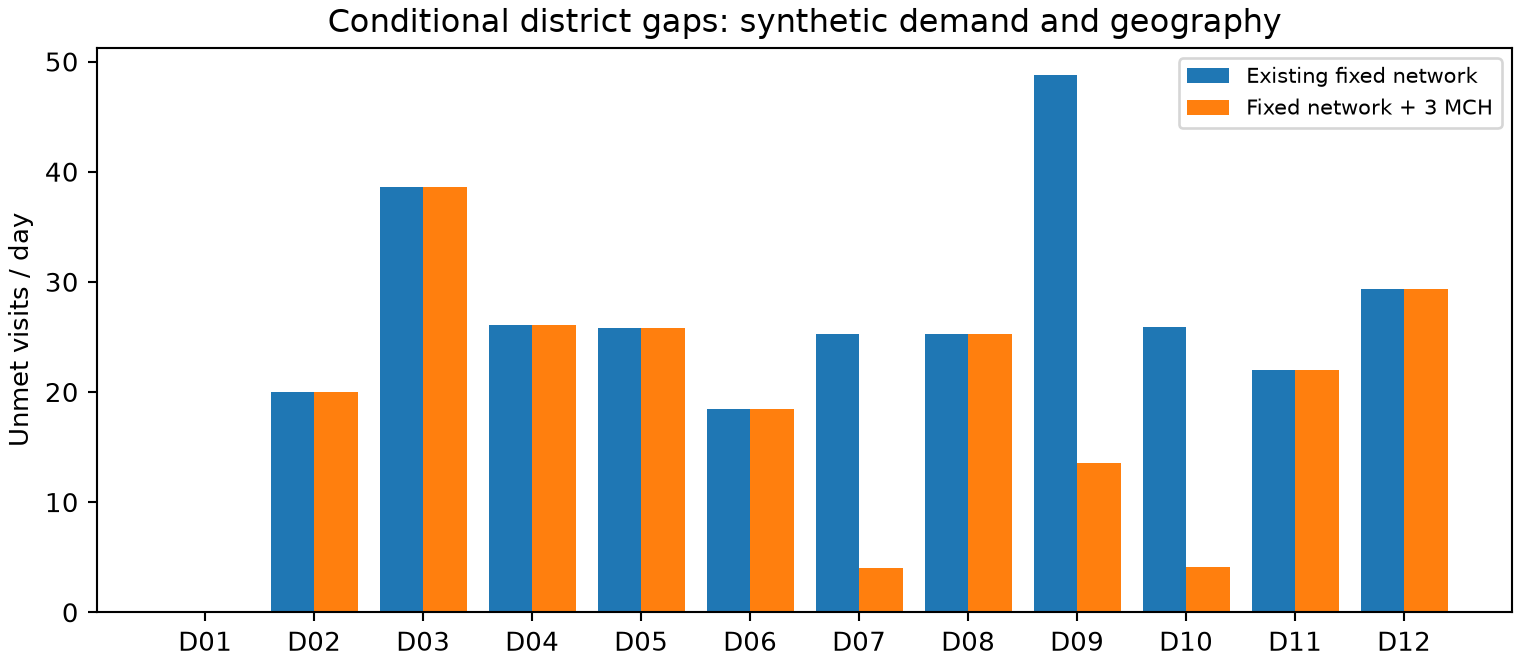
\includegraphics[width=0.88\textwidth]{results/takeover_20261120/core/district_gaps.png}
\caption{模拟区固定网络与增加三台 MCH 后的条件未满足量。单位为人次/代表日，非独立居民人数；由 Python 按冻结模型 CSV 绘制，Codex 协助编辑绘图脚本，未使用生成式图像。}
\label{fig:gaps}
\end{figure}

\section{问题二：公平选址与边际收益}

\subsection{效率前沿}
表 \ref{tab:frontier} 给出合成基准下的效率选址结果。p=3 时点集为 MCH-3、MCH-7、MCH-8，边际多增加一台的改善为 21.252 人次/日；p=7 到 p=8 没有额外服务。这里的饱和仅对应当前需求、模拟点和可达矩阵。

\begin{table}[H]
\centering
\caption{枢纽数量与条件未满足量}
\label{tab:frontier}
\begin{tabular}{rrrrl}
\toprule
枢纽数 $p$ & 未满足量 & 覆盖率 & 新增一台边际改善 & 最优点集变化 \\
\midrule
0 & 305.511 & 39.5\% & -- & -- \\
1 & 270.286 & 46.5\% & 35.225 & MCH-3 \\
2 & 248.547 & 50.8\% & 21.739 & MCH-3, MCH-8 \\
3 & 227.295 & 55.0\% & 21.252 & MCH-3, MCH-7, MCH-8 \\
4 & 206.097 & 59.2\% & 21.198 & MCH-3, MCH-4, MCH-7, MCH-8 \\
6 & 168.631 & 66.6\% & 18.625 & 含 MCH-3--8 中六点 \\
7 & 154.214 & 69.5\% & 14.417 & 不含 MCH-1 \\
8 & 154.214 & 69.5\% & 0.000 & 全部候选点 \\
\bottomrule
\end{tabular}
\end{table}

\subsection{公平性与敏感性}
在 p=2 时，效率方案未满足 248.547 人次，max-min 方案未满足 262.520 人次；排除预先声明的 D08 后，max-min 最差区未满足率为 0.575，而效率解对应的非豁免最差率为 1。p=3 起，两类目标的已测结果相同。故本模型在 p=2 展示了效率与公平之间的取舍；不能沿用旧稿“所有 p 都不存在取舍”的概括。排除 D08 的指标必须与全区最差率 1.0 并列报告。

单因素扫描显示，需求尺度从 2 增至 3 时，未满足量从 482.193 增至 814.653，最优点集由 MCH-3/MCH-7/MCH-8 变为 MCH-3/MCH-4/MCH-8；无家可归者份额从 0.5 增至 0.7 时，未满足量从 227.295 增至 246.298，点集也改变。固定中心日容量从 20 增至 50 时选址改变，说明容量假设会影响策略排序。

\begin{figure}[H]
\centering
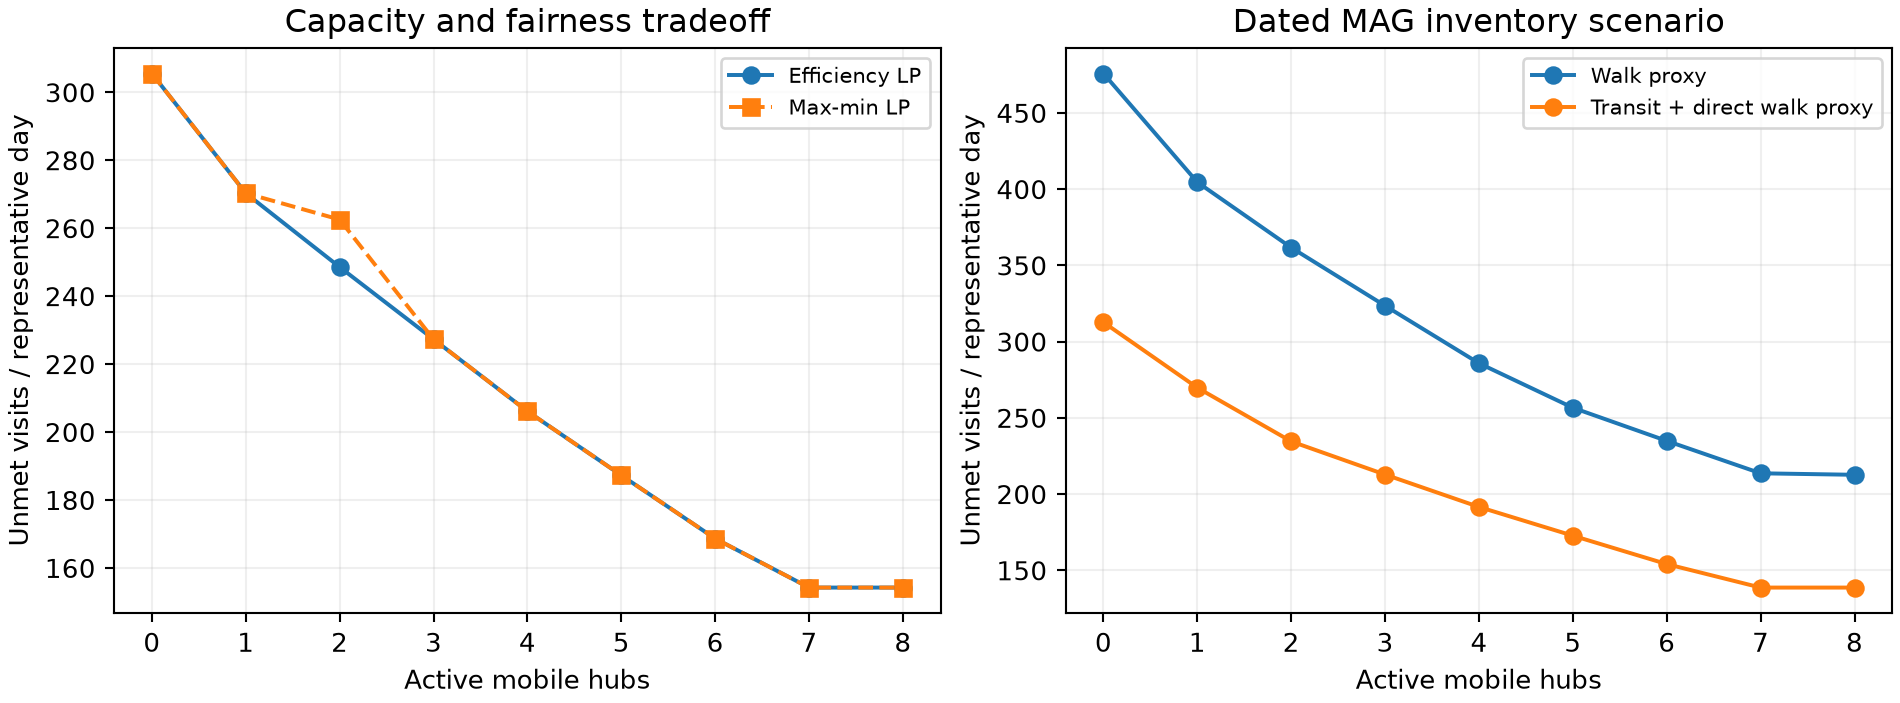
\includegraphics[width=0.92\textwidth]{results/takeover_20261120/core/frontiers.png}
\caption{候选枢纽数量前沿与 MAG 来源日历情景对照。由 Python 按冻结 CSV 绘制，Codex 协助编辑绘图脚本；右图不是独立现场服务验证。}
\label{fig:frontiers}
\end{figure}

\section{问题三：七日热浪调度}

服务日按当地 09:00 至次日 09:00 定义，夜间为 22:00 至次日 09:00；跨夜营业窗口与相邻日历求交。起始部署当日视为已就绪，每台移动枢纽需要可并行工作的司机和搭建团队；模型旅行时间为坐标距离/假定车速加 0.5 小时搭建时间。

合成基准中，固定和动态方案累计未满足量均为 1768.428 人次，最优部署七天均为 MCH-3、MCH-7、MCH-8。需求只按同一日系数整体变化时，空间相对排序不变，因此搬迁收益为零。局部冲击会改变结论：若 D05 在第 3--5 日需求乘以 3，固定方案累计缺口为 1898.683，动态方案为 1887.981，改善 10.702 人次/七日。该结果只在给定候选点、旅行代理和团队规则内最优，不能外推到真实道路或人员调度。

MAG 日期日历情景则得到固定方案累计缺口 1700.665、动态方案 1679.511，局部最优移动减少 21.154 人次/七日。动态时点为第 6 日和第 7 日。与合成基准并列报告说明移动收益取决于需求空间结构与设施营业日历，而非所有热浪均无搬迁价值。

\section{问题四：中断响应与不确定性}

\subsection{响应设计与确定性案例}
中断模型固定事故前部署，对同一故障、需求冲击、乘客可达性和搬迁耗时输入，比较不搬和可执行的重调度。默认 MAG 日历情景中，D09 与 D03 需求乘以 1.8，MAG0145 场地关闭；不搬未满足 280.897 人次，重调度至 MCH-2/MCH-3/MCH-4 后为 275.703，净改善 5.194 人次/服务日，就绪时间 1.45 小时。全区最差未满足率仍为 1.0。此数值为离散模型结果，不包含真实路况、供电、许可和团队到位观测。

另一合成车辆故障案例中，MCH-3 车辆故障、需求乘数 1.0 时不搬缺口为 262.520，精确响应为 248.547，改善 13.973 人次/日；需求乘数 1.8 和 3.0 时，改善分别为 43.681 与 86.970。场地失效与车辆失效分别建模，不混为一类事件。

\subsection{配对压力测试}
对 100 个假设抽样，逐次同步扰动故障、需求预测尺度（0.8/1/1.2）、乘客出行时间尺度（1/1.5/2）及搬迁耗时尺度（1/1.5/2），并以同一次抽样的不搬方案为基准。响应收益 P10/P50/P90 为 0/0.487/21.655 人次/服务日，59\% 抽样的响应收益为正。所有抽样存在截止内可行动作，但由于不搬或闲置始终可行，100\% 可行份额只是动作可行性检查，不是现实可靠率或 24 小时恢复概率。抽样概率和倍率是 ASSUME，未由现场故障残差估计。

\section{问题五：五年投资与运营策略}

\subsection{条件年度规划}
五年规划把拥有库存、购买和当年开工区分。每年枚举购买数量、在役数量、延时合同和接驳情景，约束完整年度费用不超过预算。默认单价为每台购置 80,000 美元、每台运营 120,000 美元、延长至 21 时为 1.5 百万美元、延长至 22 时为 2.5 百万美元、接驳为 0.4 百万美元；以上均为情景成本而非 Phoenix 报价。预算不结转，延时和接驳合同可按年取消，闲置资产保留且暂不计储存费。

base/base 情景初始拥有 3 台、年度预算 4 百万美元。DP 的第一年选择开工 4 台、购买 1 台、延长至 22 时、不接驳；第二、三年各购买并启用一台，最后两年维持 6 台。每年成本分别为 3.06、3.18、3.30、3.22 和 3.22 百万美元，均在设定预算内。五年加权未满足分数为 568.264，五个代表日均值为 113.653 人次。该结果来自已知完整热路径的有限状态 DP；代表日权重默认 1，不能称作年度客流预测。

\begin{table}[H]
\centering
\caption{预算与热浪情景下的五年对照分数}
\label{tab:q5}
\small
\begin{tabular}{lrrrr}
\toprule
预算/热路径 & DP 缺口分数 & 滚动策略 & DP 相对滚动改善 & 现有资产基线 \\
\midrule
low/mild & 583.091 & 598.170 & 15.078 & 1260.134 \\
base/mild & 537.921 & 537.921 & 0.000 & 1260.134 \\
high/mild & 537.921 & 537.921 & 0.000 & 1260.134 \\
low/base & 622.948 & 642.266 & 19.318 & 1317.300 \\
base/base & 568.264 & 568.264 & 0.000 & 1317.300 \\
high/base & 568.264 & 568.264 & 0.000 & 1317.300 \\
low/severe & 768.239 & 799.640 & 31.401 & 1493.768 \\
base/severe & 677.452 & 677.452 & 0.000 & 1493.768 \\
high/severe & 677.452 & 677.452 & 0.000 & 1493.768 \\
\bottomrule
\end{tabular}
\end{table}

\subsection{解释边界与修订信号}
base/high 路径下 DP 与滚动策略相同，low 预算下完整未来信息的 DP 有小幅改善；这不证明预算在现实中不重要，因为成本均是假设，且 DP 预知未来。成本敏感性从 MCH 成本 0.5 倍到 10 倍时，首年车队动作从启用 4 台变化为启用 2 台，最终缺口分数也上升，显示采购建议对成本敏感。

建议每年监测逐小时到访、排队与拒绝服务、实际开关门、故障恢复时间、关键区可达率、人员配置和完整年度报价。出现持续夜间缺口、热浪路径超出当前情景、候选站许可或供电变化、实际容量偏离假设或报价跨越敏感性区间时，应重新计算方案。触发复核不等于自动采购。

\section{验证、敏感性与局限}

\subsection{数值和输入核验}
冻结数值源代码提交为 \texttt{d070f5d3a90929836d210f4e6002c9dbc00a8449}。该提交记录 94 项测试通过、7 项因依赖预先运行 Q5 保存结果而跳过、1 条警告。结果 manifest 保存源代码、输入文件指纹、参数和运行环境。19 人次手算分配反例、Q3 全路径枚举、Q4 截止与车队语义反例、Q5 有限状态对照用于检验所述离散模型实现。

输入核验包括 50 个 MAG 站点 ID 的源数据对照、350 个站点—日期日历格检查、官方 15 村人口/年龄聚合守恒，以及缺失无车数据不插补。它们证明来源处理和约束实现可追溯，不证明需求预测、覆盖率或实际服务有效。服务结果留出验证状态仍为 NOT AVAILABLE。

\subsection{结果敏感性}
\begin{itemize}
    \item 需求尺度 2 到 3 倍之间，抽样点集发生变化；不能声称需求同比改变时选址排序必然不变。
    \item 无家可归者需求份额 0.5 到 0.7 之间，最优组合变化；访客样本比例仅提供背景。
    \item 固定站容量 20 到 50 人次/日时，点集发生变化；容量不确定会改变推荐布局。
    \item 步行代理阈值从 20 到 45 分钟时，当前合成解保持不变；60 分钟时未满足量下降，但并不识别真实步行时间。
    \item 延长营业时间、移动枢纽数量和成本共同影响服务路径。单因素结果不表示社会因素的因果效应。
\end{itemize}

\subsection{主要限制}
\begin{enumerate}
    \item 潜在需求和未到访需求没有独立调查。历史访问会受到营业时间、交通、宣传和容量截断影响。
    \item 逐站真实日容量、小时吞吐率和拒绝服务记录缺失；容量假设能改变选址。
    \item 区中心和距离/速度矩阵不是人口加权路网或门到门 GTFS OD，偏差方向未知。
    \item 参考 MAG 日历来自 2026 来源字段，不是 2027 真实未来运营日历；未知小时采用的处理是工作政策。
    \item 车辆并行需要多组司机/搭建人员；道路、许可、供电、无障碍和站点现场条件尚未逐项核实。
    \item Q5 成本、采购交期、持有费用、预算和未来热路径仍为假设；年度代表日评分不等同年度受益量。
    \item 没有与部署相匹配的健康结局留出数据，本文不估计对中暑、住院或死亡的因果影响。
\end{enumerate}

\section{结论与决策建议}
在当前合成基准中，3 台 MCH 提高了总服务覆盖，但全区最差未满足率仍为 100\%；这说明增加移动资源不能自动解决结构性不可达。加入 MAG 公开点位和日期化营业日历后，固定网络和移动布局的结果与合成基准不同，进一步表明交通、需求空间分布和营业时间共同决定模型答案。

模型没有证明某个固定采购数对 Phoenix 全市最优。较稳健的下一步是收集逐站真实容量、逐小时访问与拒绝服务、站点实际开门时间、完整出行链、人员和合同成本，并以试点期留出数据检验预测。决策者可先比较现有固定中心延时与小规模移动试点；仅在现场许可、供电、人员、交通和单位服务成本得到核实后，才将模拟候选转换为真实部署计划。

\section*{参考文献}
\addcontentsline{toc}{section}{参考文献}
\begin{thebibliography}{99}

\bibitem{mcm2027b}
COMAP. \emph{2027 Mathematical Contest in Modeling, Problem B: Keeping Phoenix Cool}. 2027. 本地赛题文件。

\bibitem{phoenixplan}
City of Phoenix. \emph{2026 Heat Response Plan}. 2026. 本地官方计划。

\bibitem{weeklyreport}
City of Phoenix. \emph{Phoenix Weekly Heat Reports 2025}. 2025. 本地官方周报。

\bibitem{maricopasurvey}
Gettel, A. et al. Cooling Center Use and Heat-Related Illness in Maricopa County, Arizona, 2023. \emph{MMWR}, 74(14), 252--255, 2025. doi:10.15585/mmwr.mm7414a4.

\bibitem{gtfs}
Valley Metro. \emph{GTFS Static Schedule Feeds}, 2026 summer service periods (feed snapshots mdb-147-202606160033 and mdb-147-202607280152). Effective dates 2026-04-27--07-26 and 2026-07-27--10-25; archived validation and checksums in the project repository.

\bibitem{acs}
City of Phoenix Housing and Community Development Department. \emph{2024 Neighborhood and Demographic Profile}, Appendix: urban-village population, household, and age counts derived from ACS 2018--2022, pp. 34, 37. These are report-derived counts, not the paper's simulated 12-district boundaries.

\bibitem{mag}
Maricopa Association of Governments. \emph{Heat Relief Network Public View}, Phoenix records, 2026 season; snapshot queried 2026-11-18. ArcGIS FeatureServer item and archived response/checksum listed in the project repository.

\bibitem{modelrepo}
EveyGA and team. \emph{MCM 2027 B Phoenix Cooling: source code, data, frozen experiments, and traceable handoff}. GitHub repository. \url{https://github.com/KN-1998/mcm2027-b-phoenix-cooling}.

\bibitem{comapAI}
COMAP. \emph{MCM/ICM Policy on the Use of Generative AI Tools}. Contest policy document.

\end{thebibliography}

\clearpage
\section*{致凤凰城市议会的信}
\addcontentsline{toc}{section}{致凤凰城市议会的信}

尊敬的凤凰城市议会成员：

我们评估了一个假设性的移动降温枢纽计划，重点考察居民在需要时能否到达合格的室内降温服务。模型将饮水站与降温中心分开处理，并按开放时段、代理旅行时间和服务容量计算规划服务人次。竞赛中的 12 个规划区和 8 个候选点均为模拟设定，模型数字不是 Phoenix 居民的实测覆盖率。

在当前测试中，增加移动枢纽可以改善平均服务量，但一些地区的缺口仍然存在。七日热浪下，只有局部需求冲击才使搬迁产生改善；多数应急抽样中的改善较小。五年规划对当地尚未核实的运营成本、人员、采购和资产条件较敏感。我们因此不建议仅凭本模型承诺固定采购数量或宣称可减少某个数量的热相关疾病与死亡。

建议首先核实固定中心延时开放所需的人员与运营成本，同时建立逐小时到访、排队、拒绝服务、营业状态、容量和交通信息的统一记录。之后可开展小规模移动枢纽试点，逐一核查候选场地许可、供电、无障碍、车组和实时路线。每个热季后以未参与拟合的完整服务周评估模型；若观测缺口、成本或可达条件超出已测情景，再更新方案。模型输出应作为比较和试点设计工具，而不是自动派车或采购命令。

谨致，\\
研究团队

\label{solutionlastpage}
\clearpage
\fancyhead[R]{AI 使用报告}
\section*{AI 工具使用报告}
\addcontentsline{toc}{section}{AI 工具使用报告}

本工作稿使用 OpenAI Codex 协助整理结构、核对仓库中的代码与数值结果、修订中文表述、编辑绘图脚本并编辑 \texttt{2702.tex}。图件由 Python 根据团队模型输出绘制，未使用生成式图像模型；AI 工具不构成外部观测或独立验证。提交前，团队成员必须复算关键结果、核对来源和图件，并按竞赛政策确认实际协助记录。AI 使用报告按赛题/竞赛说明单独处理，不纳入主体页数统计；最终页数以提交规则和终稿版面复核为准\citep{comapAI}。

\end{document}
